\subsection{Solidity Compatibility}\label{section: solidity-compatibility}

Solidity is an advanced programming language specifically designed for smart contract development. It is widely used on the Ethereum network and supported by other blockchain projects that are compatible with the Ethereum Virtual Machine (EVM). The following advantages of Solidity make it necessary for some blockchain projects to support it:

\begin{itemize}
    \item Solidity has a large developer community and user base, with many excellent smart contract projects and cases that can provide reference and inspiration for other blockchain projects. Supporting Solidity can attract these existing developers and users, increase their own activity and liquidity.
    \item Solidity has good compatibility and portability, which allows it to run on different blockchain platforms as well as interact with other languages and protocols such as WebAssembly, Rust, C++, etc. Supporting Solidity can reduce developers' learning costs and migration difficulties while improving their openness and flexibility.
    \item Solidity has a rich development toolset and ecosystem including compilers, debuggers, testing frameworks, code analysis tools, code libraries etc., which can improve development efficiency and code quality. Supporting Solidity enables developers to enjoy these mature tools and resources thereby enhancing their security and stability.
\end{itemize}

Therefore, some blockchain projects need to support Solidity in order to attract more developers and users; enhance their competitiveness and influence; contribute towards the development and innovation of smart contracts.


\subsubsection{How OlaVM Supports Solidity?}

The Ola compiler generates an abstract syntax tree (AST) by parsing the syntax of Solidity. In Solidity, contracts are composed of various functions. Therefore, the Ola compiler first parses the function definitions of Solidity contracts and converts each function into a corresponding AST node. For each function, the Ola compiler parses the function's parameters, return values, visibility, and other attributes, and represents them as properties of AST nodes. When parsing the function body, the Ola compiler decomposes the function body into basic statement blocks, such as assignment statements, conditional statements, and loop statements, and converts them into corresponding AST nodes. During this process, the Ola compiler performs semantic analysis to check the correctness of statements and the type matching. For example, when parsing an assignment statement, the Ola compiler checks whether the types on both sides match. If not, a compilation error is generated.

In addition to function definitions, Solidity also supports advanced syntax structures such as structures, enumerations, and events. When parsing these structures, the Ola compiler converts them into corresponding AST nodes and generates the corresponding Ola opcode. In general, the Solidity parsing process in the Ola compiler can be divided into the following steps:

\begin{itemize}
    \item Lexical analysis: Decompose Solidity code into basic lexical units (such as keywords, variable names, and numbers).
    \item Syntax analysis: Combine lexical units into an abstract syntax tree according to Solidity's syntax rules.
    \item Semantic analysis: Check the correctness and type matching of the syntax tree, and generate the corresponding Ola opcode.
\end{itemize}

After parsing, the AST tree is obtained. The process of generating LLVM IR from the AST tree includes the following steps:

\begin{itemize}
    \item The Ola compiler converts the Solidity AST nodes into corresponding LLVM IR syntax tree nodes and maps the variables, types, functions, and other information in Solidity to the types, global variables, functions, and other elements in LLVM IR.
    \item After generating the LLVM IR syntax tree, the Ola compiler optimizes it and then compiles it into Ola opcode, which is the instruction set that OlaVM can execute directly. Specifically, the Ola compiler converts the LLVM IR syntax tree into Static Single Assignment (SSA) form, where each variable is assigned only once, making it easier for subsequent analysis and optimization.
\end{itemize}

Then, the Ola compiler converts the LLVM IR syntax tree in SSA form into Ola opcode, which mainly includes the following steps:
\begin{itemize}
    \item Convert the basic blocks in the LLVM IR syntax tree into basic blocks in Ola opcode.
    \item Convert the instructions in the LLVM IR syntax tree into Ola opcode instructions. Ola opcode instructions are simpler than LLVM IR instructions and only include basic operations, branching, and jumping instructions.
    \item Convert the PHI instructions in the SSA form of the LLVM IR syntax tree into phi instructions in Ola opcode.
\end{itemize}
After completing the above process, the Ola compiler generates Ola opcode that can be executed on OlaVM. By introducing the intermediate representation form LLVM IR, the Ola compiler can compile Solidity into LLVM IR, and then compile LLVM IR into Ola opcode, making OlaVM support not only Ola language but also many programming languages that can be compiled to LLVM IR, with better flexibility and extensibility.

The above process is shown in the diagram\ref{fig:solidity-compile}.

\begin{figure}[!ht]
    \centering
    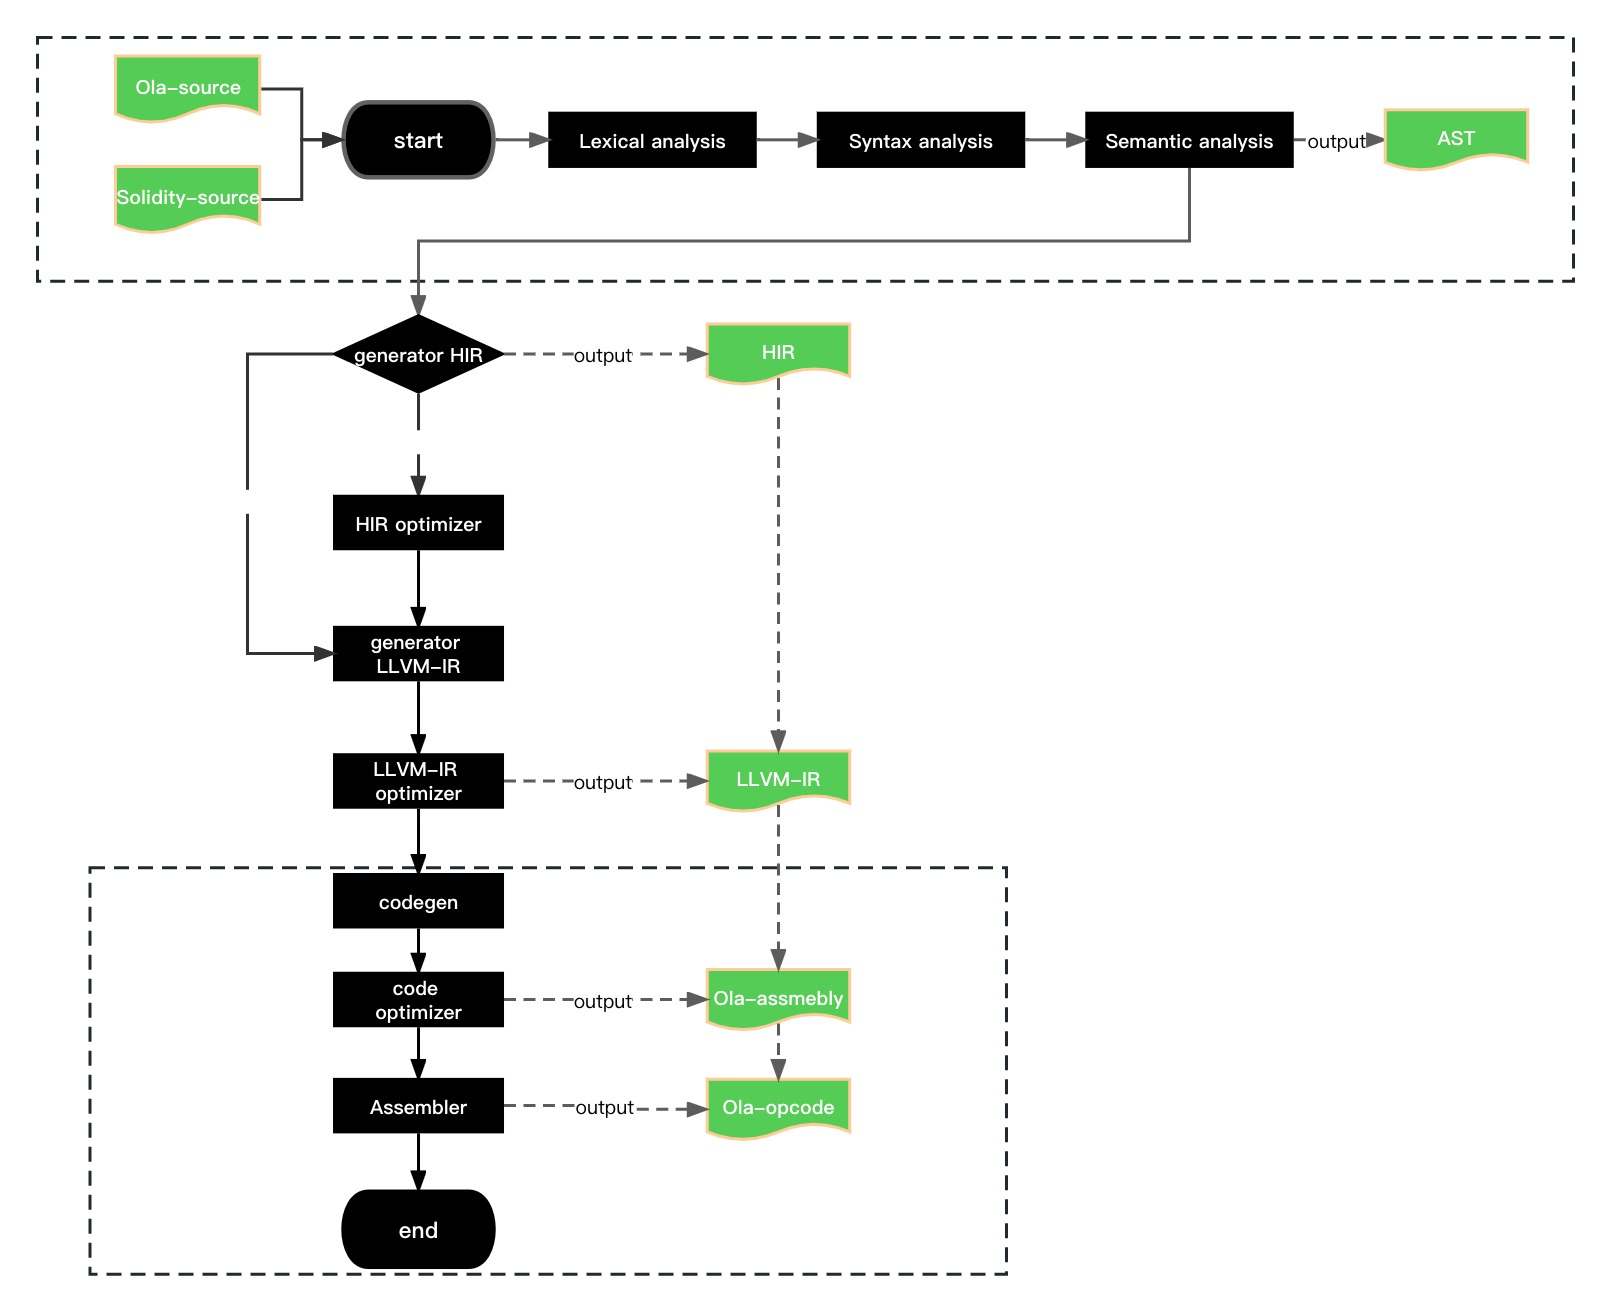
\includegraphics[width=0.6\textwidth]{images/solidity-compile.jpg}
    \caption{Solidity Compilation Process}
    \label{fig:solidity-compile}
\end{figure}

\subsubsection{Details To Be Addressed}

Although compiling Solidity into LLVM IR is feasible, there are many details in between that are worth considering. This is also a key direction that needs improvement.

\begin{itemize}
    \item Data type mapping: Solidity has many proprietary data types, such as uint, int, address, bytes, bool, etc. When converting Solidity code to LLVM IR, these data types need to be mapped to data types supported by LLVM IR.

    \item Function calls and message passing: Solidity contracts communicate with each other through message passing and support both external and internal function calls. When compiling Solidity to LLVM IR, these calls and message-passing mechanisms need to be handled correctly.

    \item Storage and memory: Solidity has two types of data storage: persistent storage and memory. The compiler needs to be able to correctly handle these storage types and map them to the corresponding data structures in LLVM IR.

    \item Exception handling: Solidity uses statements like revert, require, and assert to handle exceptions. When compiling Solidity to LLVM IR, these exception handling mechanisms need to be mapped to the exception handling structures in LLVM IR.

    \item Access control and visibility: Solidity supports access control and visibility modifiers, such as private, internal, public, and external. These modifiers need to be correctly converted to access control and visibility structures in LLVM IR.
\end{itemize}

Fortunately, some of the issues can be solved by defining certain built-in functions and built-in structures, but there are also some problems that cannot be directly resolved, such as:

\begin{itemize}
    \item EVM-specific features: Solidity has some features specific to the Ethereum Virtual Machine (EVM), such as selfdestruct, gasleft, and blockhash. These features may not be applicable to other platforms based on LLVM IR and may require alternative solutions or limitations on their use.

    \item Full ABI support: Solidity's Application Binary Interface (ABI) is used for encoding and decoding data between contracts. Compiling Solidity to LLVM IR may require additional implementation to support the full ABI.

    \item Optimization and Performance: Compiling Solidity to LLVM IR may result in performance loss, as we introduce non-deterministic computation in the Ola language. This solves most of the difficult-to-compute but easy-to-verify problem scenarios, which cannot be gained by directly processing Solidity.

    \item Platform compatibility: Different platforms may have different constraints and limitations, which may cause some Solidity features to be unsupported. When performing the conversion, these factors need to be carefully considered and adjustments made to the Solidity code as needed
\end{itemize}
